\documentclass[10pt,letterpaper]{article}
\usepackage{amsmath,amsthm,amsfonts,amssymb,amscd}
\usepackage{fullpage}
\usepackage{lastpage}
\usepackage{enumerate}
\usepackage{fancyhdr}
\usepackage{mathrsfs}
\usepackage[framed]{mcode}
\usepackage{xcolor}
\usepackage{dsfont}
\usepackage{gensymb}
\usepackage{graphicx}
\usepackage[margin=3cm]{geometry}
\setlength{\parindent}{0.0in}
\setlength{\parskip}{0.05in}

% Edit these as appropriate
\newcommand\course{CIS580}
\newcommand\semester{Spring 2015}     % <-- current semester
\newcommand\hwnum{}                  % <-- homework number
\newcommand\yourname{Michael O'Meara and Michael Woods} % <-- your name
\newcommand\hwdate{Due: April 27, 2015}           % <-- HW due date

\newenvironment{answer}[1]{
  \subsubsection*{1}
}


\pagestyle{fancyplain}
\headheight 20pt
\lhead{\yourname\ \login\\\course\ --- \semester}
\chead{\textbf{\Large Project 2 Preliminary Report \hwnum}}
\rhead{\hwdate}
\headsep 10pt

\begin{document}

\begin{enumerate}[1]
\item \textbf{Before RANSAC}

\begin{figure}[h!]
 \center
  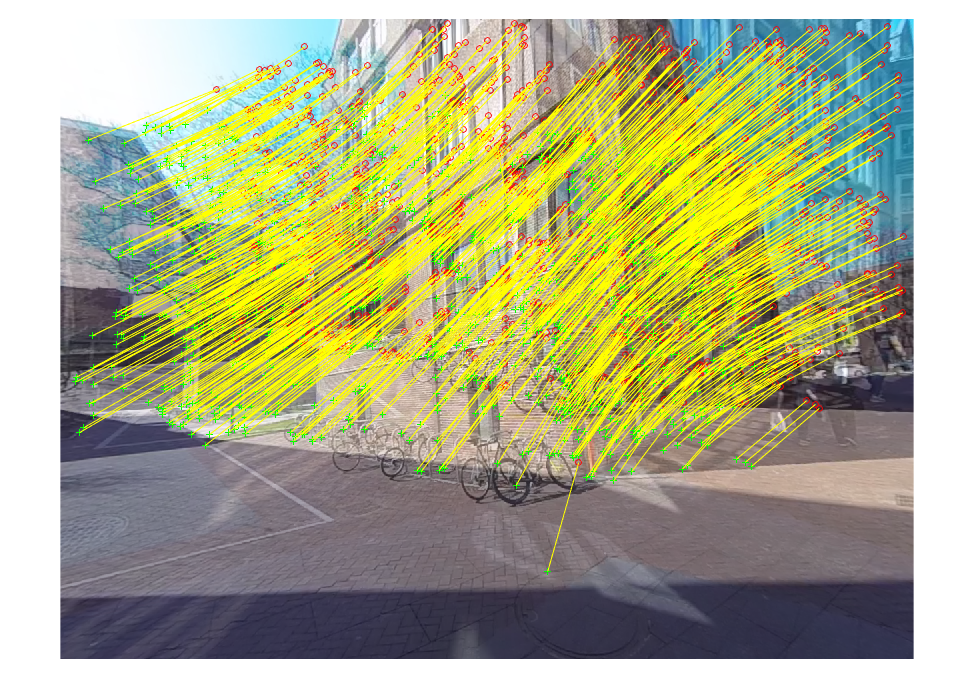
\includegraphics[width=4in]{images/before_ransac}
  \caption
   {}
\end{figure} \\

\item \textbf{After RANSAC}

\begin{figure}[h!]
 \center
  \includegraphics[width=4in]{images/after_ransac}
  \caption
   {}
\end{figure} \\

\newpage

\item \textbf{Reprojection of 3D points back to 2D image1}

\begin{figure}[h!]
 \center
  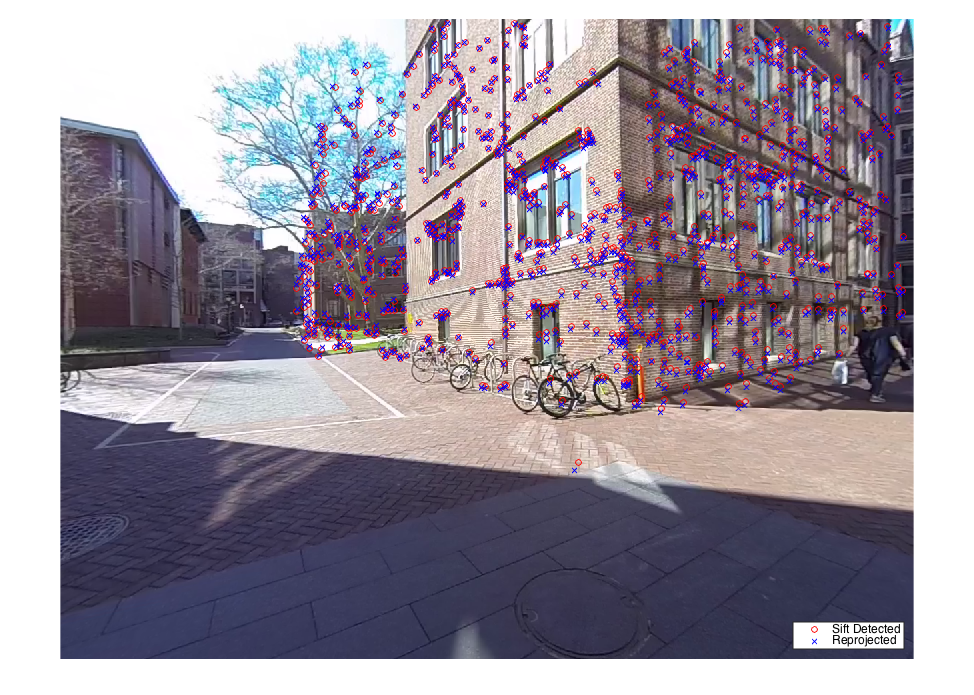
\includegraphics[width=4in]{images/reprojection_image1}
  \caption
   {}
\end{figure} \\

\item \textbf{Reprojection of 3D points back to 2D image2}
\begin{figure}[h!]
 \center
  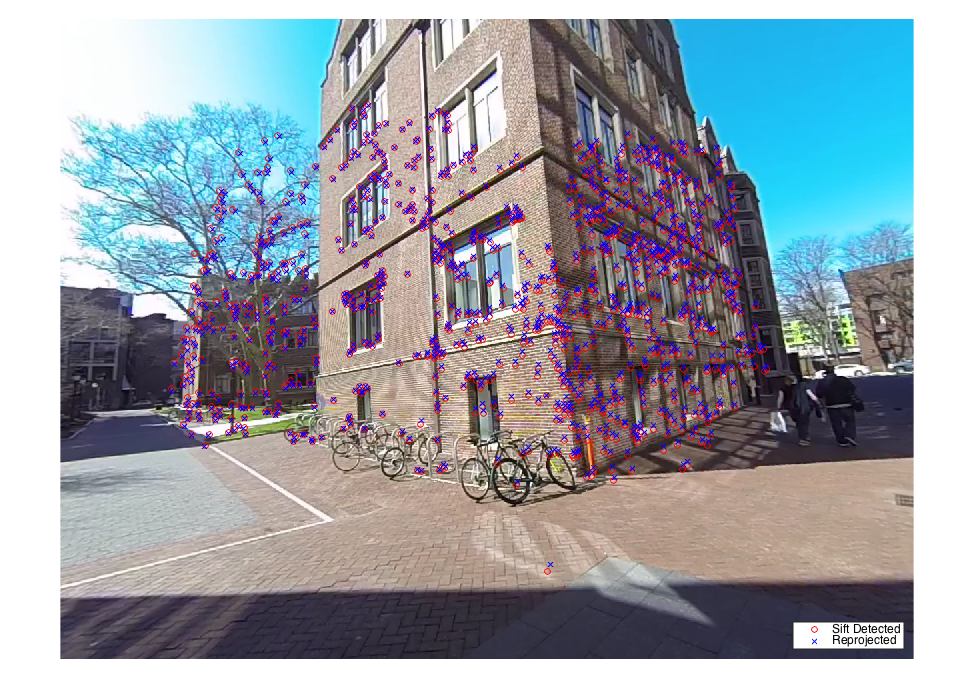
\includegraphics[width=4in]{images/reprojection_image2}
  \caption
   {}
\end{figure} \\

\newpage

\item \textbf{Triangulated 3D points}
\begin{figure}[h!]
 \center
  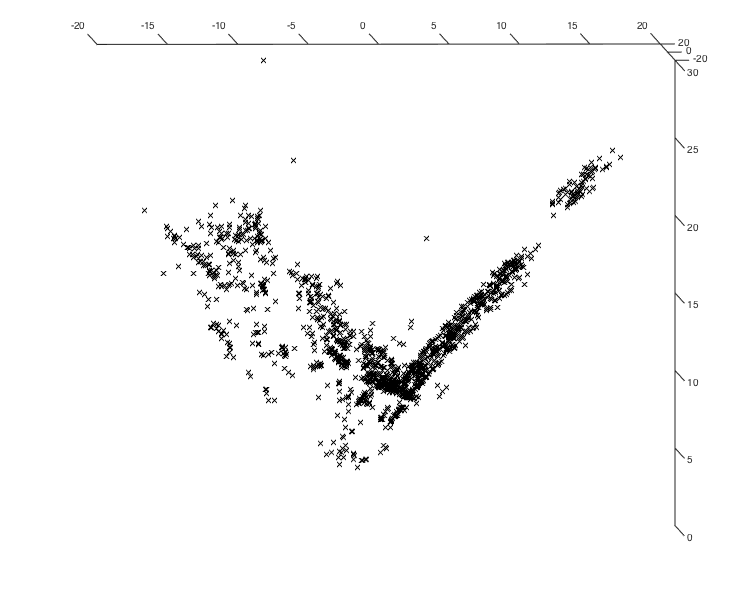
\includegraphics[width=4in]{images/3D}
  \caption
   {}
\end{figure} \\



\end{enumerate}
\end{document}
